\chapter{Besluit}
\label{besluit}

Dit project heeft een lange weg afgelegd. De initi\"ele beschrijving van de thesisopdracht ging over het maken van (innovatieve) gebruikersomgevingen om te helpen met het vinden van passende fragmentparen. De kernvraag luidde: ``welke informatie is nodig om te kunnen zeggen of een paar wel of niet past? Hoe kan die weergegeven worden? Kan dit bijvoorbeeld voor 1000 paren tegelijkertijd?'' Het zoeken naar d\'e nieuwe weergave van fragmentparen die een archeoloog in staat zou stellen om op effici\"entere wijze naar de enkele correcte paren in een zee van incorrecte voorstellen te zoeken leverde lange tijd niets op.\\

Vele evidente en minder evidente weergaven waren reeds v\'o\'or dit thesisproject te vinden in het thera project. Men kan de fragmenten op allerlei manieren bekijken. Behalve de gewone weergave in kleur valt de achterzijde te bezien, de contour alleen, de dikte, \ldots. Interessant zijn de normalen van het oppervlak die kunnen gevisualiseerd worden om een beter idee te krijgen van het reli\"ef (zo kunnen onder andere krassen en borstelafdrukken duidelijk worden). Tevens kan de doorsnede van de plaats waar beide fragmenten elkaar raken bekeken worden, dit bleek zo nuttig te zijn dat het in Browsematches en dit thesisproject standaard aan de linkerkant van een paar wordt weergegeven. E\'en mogelijke uitwerking van de thesis zou dus geweest zijn nog een alternatieve voorstelling te vinden die snelle en accurate beslissingen toelaat en bij voorkeur zeer compact (1000'en paren tegelijk) is. Helaas is het op dit vlak qua idee\"en nooit verder gekomen dan incrementele verbeteringen op de huidige resultaten (bvb. niet-lineaire doorsneden van fragment visualiseren). 

Grosso modo vallen er twee aanpakken te onderscheiden om het identificeren van paren te verbeteren: ofwel weet een algoritme de paren te rangschikken op zo'n manier dat de correcte paren eerst te zien zijn \'of men kan ervoor zorgen dat (zeer) grote deelverzamelingen in korte tijd kunnen beoordeeld worden (hoge doorvoer). Anders gezegd: gericht zoeken naar paren of ze allemaal afgaan.

De tweede aanpak krijgt echter te maken met een fundamentele limiet gebaseerd op de informatietheorie.

De twee aanpakken zijn niet logisch onderling uitsluitend, maar hoe succesvoller de eerste aanpak is des te minder impact heeft de tweede. Immers als het overgrote deel van van de correcte paren op een rij kan gezet worden zullen de weinige slechte paren het reconstructiewerk niet lang verhinderen zelfs als er helemaal niet virtueel nagekeken wordt. Vice versa geldt dit ook: als alle voorstellen op een redelijke tijd virtueel beoordeeld kunnen worden, moeten ze niet noodzakelijk in een goede volgorde staan. Kan dit echter wel? Misschien is de zoektocht naar een methode om zo snel mogelijk met het menselijke oog te verifi\"eren wel mislukt omdat er . Het is lastig om steeds \'e\'en per \'e\'en te moeten werken zoals in Griphos, maar na een zeker punt zijn er effici\"entieverliezen.
 Hoe compacter de data kan voorgesteld worden, hoe gemakkelijker het in een getal kan omgezet worden. In de limiet  

Het verschil is dat terwijl de sorteeraanpak theoretisch niet moet onderdoen voor een mens die alle brokstukken met de hand aan elkaar probeert te passen\footnote{Gegeven dat de data volledig genoeg is, resolutie is belangrijk. Dit valt te zien door in te beelden dat de resolutie zeer laag is en alle fragmenten gedigitaliseerd worden als perfecte kubussen van verschillende grootte.}, er w\'el een limiet staat op de ``doorvoersnelheid'' van het correct/niet-correct proces. Het komt erop neer dat 

maar er is een belangrijk verschil: er is een duidelijke limiet aan het ``zo veel mogelijk tegelijkertijd principe''. Eenmaal het zo klein wordt dat er comfortabel duizenden op een scherm passen, is het ook klein genoeg om accuraat naar een getal omgezet te worden (of het is reeds een getal).  simpelweg door de rekening te houden met de mogelijke informatieinhoud van een klein aantal pixels. (uitlet over throughput limiet). Gezien het feit dat er een limiet is aan deze de maximale Hiermee rekening houdend en zien dat er miljoenen paarvoorstellen zijn 

Het feit blijft dat er nog steeds geen visualisatie is die compact genoeg en toch de nodige zekerheid geeft dat een paar correct dan wel niet correct is. Een incorrect paar vinden is echter niet zo nuttig als het vinden van een incorrect paar. Dit is zo omdat 

Misschien is het niet zo gemakkelijk om te zien welke paren correct zijn, maar is het wel mogelijk om snel te zien welk zeker niet correct zijn. Dan stelt zich het probleem dat er een manier moet zijn om deze snel te selecteren en te onderscheiden van degenen die dit niet zijn.

Andere beloftevolle insteken, zoals het gebruiken van contextinformatie en menselijke input om een virtuele classificator te trainen worden reeds onderzocht door onderzoekers Antonio Garcia Castaneda (Clusters) en Tom Funkhouser (Machine Learning) respectievelijk.\\

Mijn suggestie is: dynamische herberekening met procesverloop. In de realiteit wordt de finale conclusie over een voorstel gemaakt als men de brokstukken op de aangegeven plaats aan elkaar zet en ze ``klikken''. Door de erosie over de tijden heen is de klik op zich niet altijd 100\% vast en daarom gebeurt het dat zelfs met de fragmenten in de hand een amateur nog altijd geen sluitende conclusie kan geven. Evenwel zijn er niet veel voorstellen die na deze controle twijfelgevallen blijven. Misschien is (een deel van de) oplossing om de weergave dynamisch te maken. Uit ervaring is gebleken dat mensen snel kunnen opmerken wanneer een voorstel potentieel heeft, maar niet in een oogopslag kunnen zeggen dat het zeker juist is. Deze opmerking combineren met de methode Voor deze interessante paren is het mogelijk om te doen wat voor de minder interessante niet mogelijk was. 
 De algoritmen die in het thera project gebruikt worden om paren aan elkaar te zetten zijn gemaakt met computationele effici\"entie in gedachten,
Een mens is goed in het snel opmeten van interessantheid

\begin{figure}[ht]
	\begin{center}
		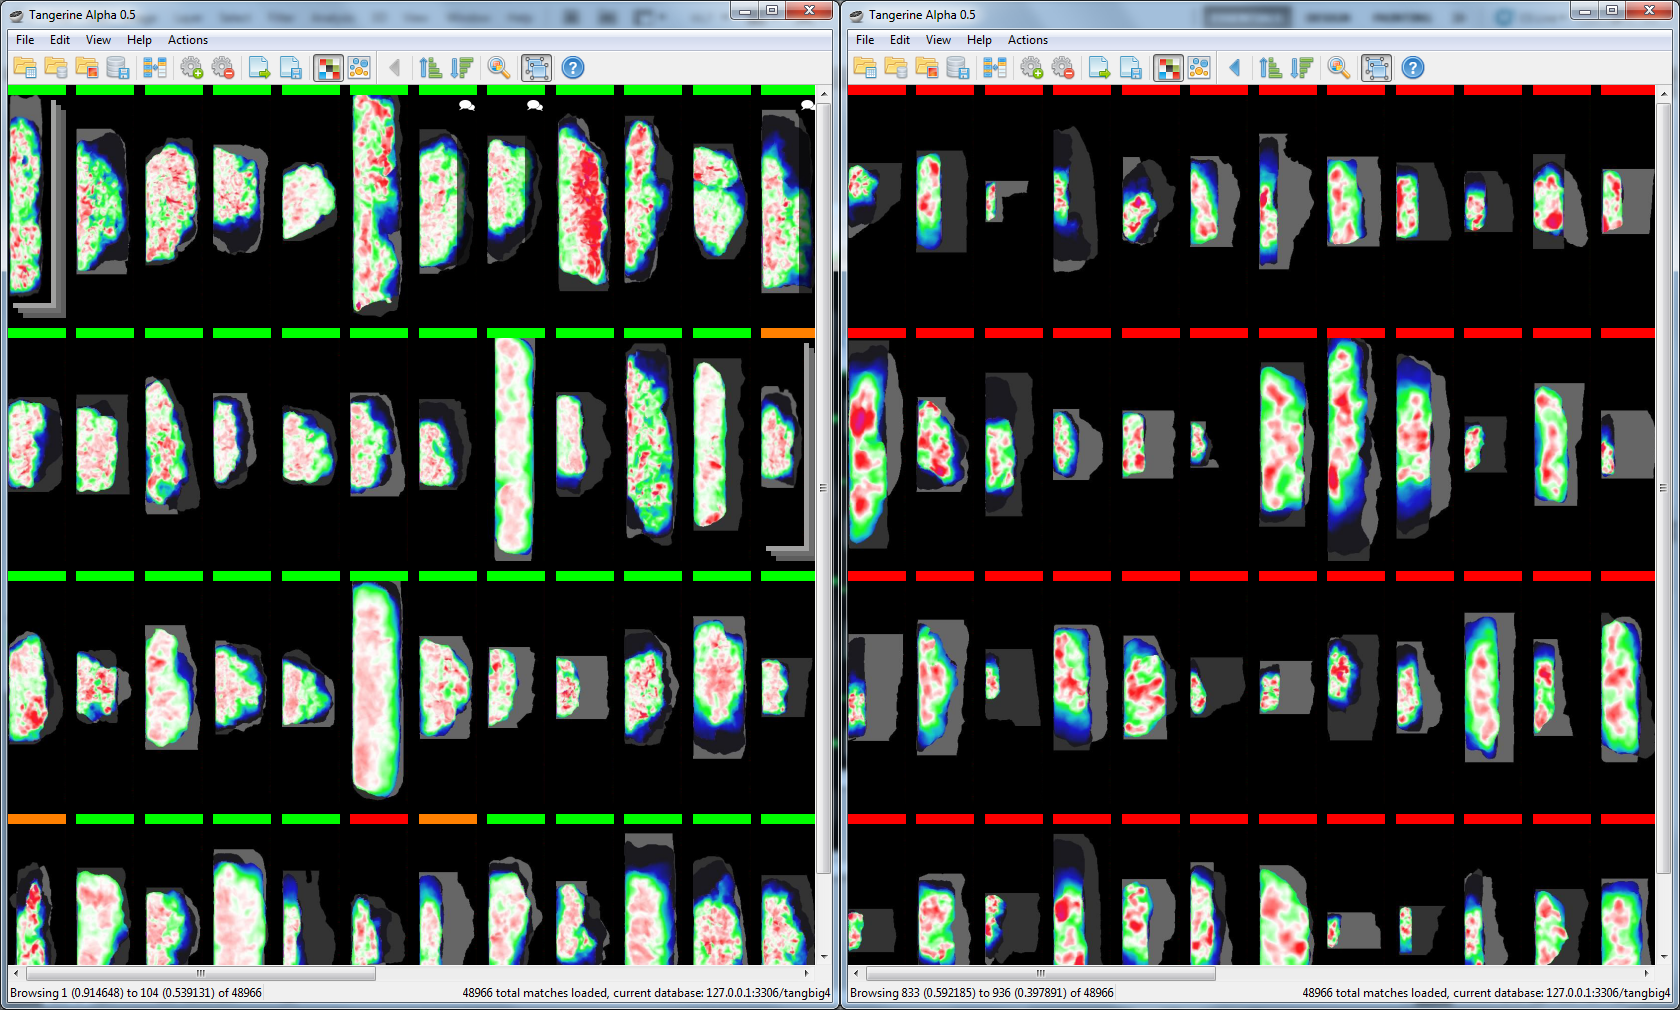
\includegraphics[width=1.0\columnwidth]{images/tileview-reduced-compare-01.png}
		\caption{De doorsnedes van goede paren tegenover die van slechte paren. Een mens kan met ervaring leren om hieruit reeds veel af te leiden. Yassine Ryad bewees dat een algoritme kan gemaakt worden dat deze informatie in een rangschikking omzet.}
		\label{fig:tileview-reduced-compare}
	\end{center}
\end{figure}

Waarschijnlijk komt dit omdat het niet de juiste insteek is. Er is een maximale informatiedensiteit. Het bekijken van een enorme hoeveelheid aan paren tegelijkertijd Niettemin zou het kunnen dat er inderdaad een visualisatie bestaat die een optimale relevante informatiedensiteit bezit. Een voorbeeld van een dense voostelling is een intensiteitsmap van zoveel mogelijk fragmentparen (stel 1 pixel per paar) waar de intensiteit gelijkgesteld wordt aan de beoordeling van een automatische herkenner of een combinatie van meerdere herkenners en menselijke input (cfr. Machine Learning). Maar hier kan een archeoloog niet zoveel meer uit leren dan gewoon te sorteren op deze karakteristiek en in die volgorde paar na paar na te kijken. Als een karakteristiek werkelijk een onderscheid kan maken tussen correcte en niet-correcte paren zal dit in ieder geval moeten gebeuren. Dit soort dense visualisaties heeft dus vooral nut voor de ontwikkelaars van de karakteristieken zelf, zij kunnen een beter overzicht krijven van de verdeling binnen de set van alle paren. Het passen van fragmenten is een complexe taak, maar niet zo complex dat het onmogelijk lijkt om een getal te plaatsen op de relatieve ``goedheid'' van een paar. Het zoeken naar zo'n getal of karakteristiek is daarom op zich een waardevolle bezigheid. Dat was echter niet het onderwerp van deze thesis, maar van een andere die in dezelfde tijd aan de K.U.Leuven werd gemaakt binnen het thera project [referentie thesis yassine].\\

In het kort zou er dus een weergave moeten gevonden worden die:

\begin{itemize}
	\item Compact is
	\item De relevante informatie bevat voor het beslissen over de correctheid van een paar
	\item Niet sorteerbaar is (dan is het probleem opgelost)
	\item Menselijke verificatie nodig heeft
\end{itemize}

Een goed voorbeeld van een voorstelling die compacter is dan het voorstellen van de paren zelf en niet sorteerbaar is, is het weergeven van de doorsnede. 

Geen revolutionaire idee\"en voor visualisaties die een thesis kunnen vullen en een heleboel reeds lopende projecten op alle vlakken, wat nu gedaan? Uit een kijk op de defici\"enties van het thera project bleek dat er aan nieuwe delen werd gewerkt maar de infrastructuur niet optimaal was om alles aan elkaar te knopen, om de resultaten bij de gebruiker te brengen. Het project klaarmaken voor een eventueel nieuw paradigma en het toegankelijker maken van de informatie die reeds beschikbaar was, werden het nieuwe doel.\\

Net zoals een gebroken fresco in feite een puzzel is, kan men het thera project zien als de som van vele delen die in elkaar passen. Dit thesisproject is bedoeld als een stuk dat een ander perspectief biedt op het geheel en het in staat moet stellen om meer en sneller resultaten te boeken. Het complementeert de bestaande aanpakken en zorgt ervoor dat de resultaten van de automatische paarherkenning nog nuttiger gebruikt kunnen worden. Omdat het finale validatiewerk noodzakelijk door mensen moet gebeuren, is het geproduceerde werk waardevol: het kan niet zonder meer opnieuw door een algoritme gegenereerd kan worden. De voor dit thesisproject gemaakte componenten proberen er onder andere voor te zorgen dat het verlies van informatie zo min mogelijk voorkomt door robuuste dataopslag en synchronisatie mogelijk te maken.\\

Op het vlak van ontginning van nuttige informatie met nieuwe visualisaties en nieuwe manieren om de juiste patronen te ontdekken zijn er natuurlijk nog steeds vele opportuniteiten. Want --- zoals opgemerkt in een recente paper over het thera project [citatie siggraph submission 2011] --- het vinden van de juiste paren is zoals zoeken naar een naald in een hooiberg. Met elke nieuwe toevoeging aan de mogelijkheden van het platform is er de kans dat deze een manier is om de hooiberg te verkleinen, door te lichten met X-stralen of gewoonweg op een grote krachtige magneet in een windtunnel te plaatsen. Naar deze laatste methode is iedereen natuurlijk op zoek. Tot dan is het zeker belangrijk dat men gemakkelijk kan experimenteren alsook bijhouden en opvragen welk deel van de berg reeds doorkamt is, waar de gevonden naaldrijke aders zitten en wat hun eigenschappen zijn. Misschien zijn de naalden immers niet van metaal\ldots